\documentclass{article}
\usepackage{iclr2027_conference,times}

\input{math_commands.tex}

\usepackage{graphicx}
\usepackage{caption}
\usepackage{subcaption}
\usepackage{booktabs}
\usepackage{multirow}
\usepackage{array}
\usepackage{makecell}
\usepackage{siunitx}
\sisetup{
  group-separator={,},
  group-minimum-digits=4,
  table-number-alignment=center,
  detect-weight=true,
  detect-inline-weight=math,
}
\usepackage{microtype}
\usepackage{hyperref}
\usepackage{url}
\usepackage{etoolbox}
\usepackage{wrapfig}
\usepackage{placeins}
\usepackage{amsmath}
\usepackage{amssymb}
\usepackage{amsfonts}
\usepackage{bbm}
\usepackage{xspace}
\usepackage{xcolor}

% Float spacing
\setlength{\textfloatsep}{8pt plus 2pt minus 2pt}
\setlength{\floatsep}{8pt plus 2pt minus 2pt}
\setlength{\intextsep}{8pt plus 2pt minus 2pt}
\setlength{\abovecaptionskip}{2pt}
\setlength{\belowcaptionskip}{2pt}
\captionsetup{skip=2pt,font=small}

% Float placement
\renewcommand{\topfraction}{0.92}
\renewcommand{\bottomfraction}{0.75}
\renewcommand{\textfraction}{0.06}
\renewcommand{\floatpagefraction}{0.75}
\setcounter{topnumber}{4}
\setcounter{bottomnumber}{3}
\setcounter{totalnumber}{6}
\captionsetup[subfigure]{skip=1pt,font=small}
\captionsetup[subtable]{skip=1pt,font=small}
\setcounter{topnumber}{2}
\setcounter{bottomnumber}{2}
\setcounter{totalnumber}{4}
\renewcommand{\bottomfraction}{0.65}
\renewcommand{\floatpagefraction}{0.85}

% Style macros aligned with prior papers
\newcommand{\method}{\textsc{ChartMind}\xspace}
\newcommand{\probe}{\textsc{ProbeBench}\xspace}
\newcommand{\stitle}[1]{\noindent\textbf{#1}}
\newcommand{\ie}{{\em i.e.,}\xspace}
\newcommand{\eg}{{\em e.g.,}\xspace}
\newcommand{\wrt}{\emph{w.r.t.}\xspace}
\definecolor{tagblue}{RGB}{50,100,220}
\definecolor{tagred}{RGB}{220,50,50}
\definecolor{taggreen}{RGB}{50,140,60}

\title{Charts as Epistemic Actions for Experience-Driven Agentic Data Analysis}

\author{Anonymous Authors}

\begin{document}

\maketitle

\begin{abstract}
Data agents built on ReAct-style loops now execute complex analytical workflows over structured data, yet their intermediate reasoning still runs almost entirely through text. Human analysts instead move between numbers, tables, and charts, reading visual evidence to expose trends and anomalies that text summaries drop. We ask whether charts can serve as internal epistemic actions inside a data agent's reasoning loop, and how to teach an agent to use them. We first build \probe{}, a suite of 200 controlled tasks under four matched interface conditions, and find a persistent gap between what agents can read and what they choose to use. Agents score as well from self-generated charts as from numeric output, yet plotting access alone does not translate into consistent use. Task slices show that charts lead on temporal, pattern, and anomaly reasoning, while text leads on precise reading and conditional verification. We then propose \method{}, which distils two families of experience from conditioned trajectory rollouts. One family records how to select and verify analytical operations, and the other records when to invoke text, charts, or both. A trajectory judge scores outcomes and labels intermediate steps, and a validation gate admits only experience that improves held-out performance. On three held-out benchmarks with six LLM backbones, \method{} raises analytical accuracy and visual evidence quality over matched baselines, and backbones that never drew charts begin using them, all without touching model parameters.
\end{abstract}

\section{Introduction}
\label{sec:introduction}

\noindent Data agents translate an analytical goal into a sequence of grounded actions and derive insights step by step. Recent progress in ReAct-style reasoning and acting loops \citep{yao2023react} has enabled these agents to plan, execute, inspect, and revise increasingly complex workflows over structured data. Analytical report generation, long-horizon exploration, and exact-answer analysis all now sit within their reach \citep{lei2025dacomp,liu2026ddrbench,jing2024dsbench}. The agent operates textual analytical actions competently.

\noindent Human analysts, in contrast, do not think only in text. They move continually between numerical summaries, tables, and charts, using visual evidence to expose trends, distributions, and anomalies that a scrolling table hides. A well-chosen chart at the right moment can reshape the next step of analysis. Charts thus act as epistemic actions in the analyst's loop, and not as post-hoc report artefacts. We therefore ask whether an agent should also treat charts as intermediate evidence and learn when to invoke them.

\noindent Existing methods address only part of this decision. Chart-generation methods optimise visualisations requested by a user or an agent \citep{dibia2023lida,yang2024matplotagent,yang2025chartmimic,namgoong2025amace,lu2026multivisagent,wang2025chartoptimiser}. Chart-understanding methods assume that a chart is already available and focus on extracting information from it \citep{masry2023unichart,han2023chartllama,xu2023chartbench,liu2023deplot,liu2023matcha,zhang2024tinychart}. Recent representation-choice studies pick among predefined formats or attach visual tools with fixed rules \citep{kaur2026chartagent,das2025chartsofthought,zhou2025fres,ho2026formatmatters,xing2026tabledart,lin2026evidfuse}. In these designs, chart use is fixed at setup, tied to a specific agent, or decoupled from the current analysis state, so representation choice stays outside the analytical loop.

\noindent To turn this open question into a concrete study, we build \probe{}, a probe suite of 200 tasks synthesised from InsightBench \citep{sahu2025insightbench} with four matched interface conditions and a common ReAct backbone. Three findings emerge. First, charts alone already sustain end-to-end analysis. Second, plotting access alone does not translate into consistent use. Third, charts and text behave as complementary evidence across task slices, with charts stronger on temporal, pattern, and anomaly reasoning and text stronger on precise reading and conditional verification. These findings motivate a method that turns representation choice into a learned behaviour of the agent.

\noindent We propose \method{}, an experience-driven method that teaches a data agent to use charts inside the analytical loop. For each \probe{}, \method{} generates diverse trajectories under different representation conditions and uses $f_{\mathrm{score}}$ and $f_{\mathrm{attr}}$ to score outcomes and label intermediate decisions. A builder agent distils the labelled trajectories into two experience families. Analysis experience $\mathcal{E}_{\mathrm{ana}}$ records how to select and verify analytical operations, and representation experience $\mathcal{E}_{\mathrm{repr}}$ records when and how to invoke text, charts, or a mixture. Candidate packages are accepted only when a validation gate confirms that held-out performance strictly improves. On downstream tasks the data agent reads a frozen package as external memory, so representation choice becomes part of the analytical policy without changing model parameters.

\noindent Our main contributions are as follows.
\begin{itemize}
\item \textbf{Probe study of chart use.} We construct \probe{} with four matched interfaces and six backbones. The suite exposes a capability utility gap in current data agents and quantifies where charts and text serve as complementary evidence.
\item \textbf{Experience-driven method for chart use.} We propose \method{}. Given conditioned trajectory rollouts, it distils analysis and representation experiences under outcome scoring and step-level attribution, and only experiences that pass a validation gate enter the frozen package. \method{} is the first framework that treats charts as internal epistemic actions of a data agent through learned experience.
\item \textbf{Consistent gains on held-out benchmarks.} On DAComp-DA, DDR-Bench, and DSBench with six LLM backbones, \method{} raises analytical accuracy and visual evidence quality over matched baselines. Backbones with weak representation-selection habits begin using charts, and the results stay stable under ablations on rollout diversity, validation gating, and experience type.
\end{itemize}

\section{Charts in the Analytical Loop}
\label{sec:probe}

\noindent This section studies whether charts carry genuine analytical value for data agents and how their utility differs from text. To this end we design a controlled probe \probe{} and evaluate representative agents under four matched interface conditions. We report task construction, evaluation protocol, and three empirical findings.

\subsection{Probe Design}
\label{sec:probe-setup}

\stitle{Task construction.}\quad To isolate how intermediate representations affect agent reasoning, we synthesise \probe{} from InsightBench \citep{sahu2025insightbench}, which provides enterprise tables, open-ended questions, executable reference analyses, and target insights. We treat each valid insight as an independent task and obtain 200 \probe{} tasks. Each task contains a raw CSV table, a dataset description, an analytical question, a reference analysis, and a target insight. The agent receives the table, question, description, schema, and first three rows, and must select and execute analytical operations to produce a natural-language answer, while the target insight remains hidden for evaluation.

\stitle{Analytical dimensions.}\quad To support fine-grained slicing without leaking labels to the agent, we annotate each task along two complementary dimensions. \textit{Question type} describes the requested answer form, covering numeric lookup, composition, ranking, group comparison, temporal change, relationship, anomaly, diagnosis, and prediction. \textit{Cognitive load} describes the primary operation the analyst must perform, covering locate, scan and select, compare, pattern recognition, relational interpretation, multidimensional integration, and conditional reasoning. An LLM proposes an initial label and a human annotator verifies it. These labels support post-hoc slice analysis only and never enter the agent's context.

\stitle{Agent interfaces.}\quad To hold everything but the analytical interface constant, all four settings share a vanilla ReAct agent with one general-purpose Bash tool. Each call starts a fresh process, files persist in a shared working directory, and the CSV is exposed read-only. We fix the model, initial context, interaction limit, and tool budget across conditions. \textbf{No-tool} removes execution tools. \textbf{Text-only} exposes stdout and stderr but forbids plotting. \textbf{Chart-only} exposes generated images and stderr while hiding stdout. \textbf{Free-style} returns stdout, stderr, and images and allows both text and charts.

\stitle{Evaluation.}\quad To obtain comparable scores across settings, a shared LLM judge grades each answer against the target insight on a normalised $[0,100]$ scale. Slice analyses use task-paired differences with clustered bootstrap intervals \citep{efron1993bootstrap} and randomisation tests. Figure~\ref{fig:four-condition} and Table~\ref{tab:model-bias} summarise the two views used in the following analysis.

\begin{table}[t]
\centering
\begin{minipage}[t]{0.32\textwidth}
\centering
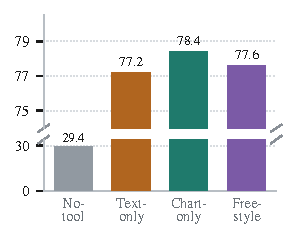
\includegraphics[width=\linewidth]{figures/interface_ablation.pdf}
\captionof{figure}{Judge scores under four matched \probe{} interfaces. The score axis is split.}
\label{fig:four-condition}
\end{minipage}\hfill
\begin{minipage}[t]{0.66\textwidth}
\centering
\small
\captionof{table}{Representation choice under \textbf{Free-style} across six backbones. \textit{Both} counts tasks that use text and charts jointly.}
\label{tab:model-bias}
\setlength{\tabcolsep}{3.2pt}
\renewcommand{\arraystretch}{1.05}
\begin{tabular}{@{}lcccccc@{}}
\toprule
\multirow{2}{*}[-0.15em]{LLM backbone} &
\multirow{2}{*}[-0.15em]{Score} &
\multicolumn{3}{c}{Representation use} &
\multicolumn{2}{c}{Interaction cost} \\
\cmidrule(lr){3-5}\cmidrule(lr){6-7}
& & Text & Chart & Both & Rounds & Tokens \\
\midrule
Claude Opus 5       & 83.1 & 43  & 0 & 157 & 3.9 & 17.4k \\
Claude Sonnet 5     & 79.2 & 102 & 0 & 98  & 4.0 & 18.7k \\
GPT-5.6 Luna        & 76.2 & 198 & 0 & 2   & 3.1 & 6.8k  \\
GPT-5.6 Sol         & 77.6 & 198 & 0 & 2   & 2.9 & 6.4k  \\
DeepSeek V4.1 Flash & 80.2 & 143 & 0 & 57  & 6.2 & 30.1k \\
HY4 Preview         & 73.1 & 198 & 0 & 2   & 3.8 & 7.7k  \\
\bottomrule
\end{tabular}
\end{minipage}
\end{table}

\subsection{Empirical Findings}
\label{sec:probe-findings}

\stitle{Finding 1. Charts alone already sustain end-to-end analysis.}\quad To check whether charts carry enough evidence for analytical questions, we compare the four interfaces under the same backbone. Figure~\ref{fig:four-condition} shows that removing execution tools collapses the agent to a low score, while text and chart interfaces bring performance close to each other. Chart-only slightly leads text-only, so the agent can read charts it just drew and extract answers of comparable quality to reading numeric tables. Charts already satisfy the sufficiency condition for intermediate evidence, so the remaining question is whether agents actually use them.

\stitle{Finding 2. Representation choice is model-dependent, not capability-driven.}\quad To probe whether the sufficiency of charts translates into use, we let each backbone freely choose between text and charts under the same Free-style interface. Table~\ref{tab:model-bias} shows large behavioural divergence. Claude Opus 5 combines text and charts on most tasks, DeepSeek V4.1 Flash on more than a quarter, while GPT-5.6 Luna, GPT-5.6 Sol, and HY4 Preview essentially fall back to text. Chart-use frequency does not track score. This shows that identical tool access yields inconsistent representation habits and confirms a capability utility gap. A method that closes this gap should shape when and how charts enter the loop, and cannot stop at exposing plotting tools.

\begin{figure}[!t]
\centering
\begin{subfigure}[t]{\linewidth}
\centering
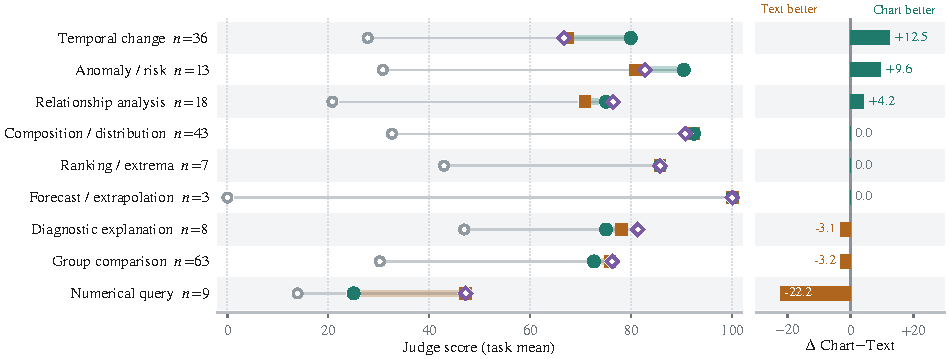
\includegraphics[width=0.9\linewidth]{figures/probe_slices_dotplot_v3_a.pdf}
\caption{Slices by question type.}
\label{fig:probe-slices-a}
\end{subfigure}
\begin{subfigure}[t]{\linewidth}
\centering
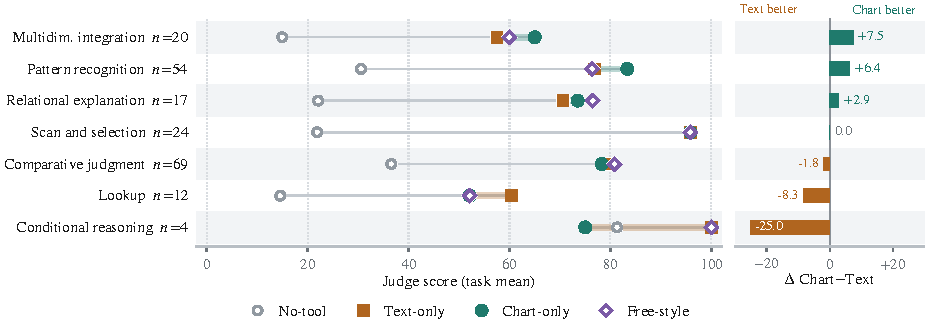
\includegraphics[width=0.9\linewidth]{figures/probe_slices_dotplot_v3_b.pdf}
\caption{Slices by primary cognitive load.}
\label{fig:probe-slices-b}
\end{subfigure}
\caption{Slice analysis of the four \probe{} interfaces. Markers show slice mean scores. The right column reports the Chart minus Text gap.}
\label{fig:probe-slices}
\end{figure}

\stitle{Finding 3. Charts and text play complementary roles across analytical tasks.}\quad To locate where each representation helps, we slice results by question type and cognitive load. Figure~\ref{fig:probe-slices} shows a clear pattern. Charts pull ahead on slices that demand shape reading, including temporal change, pattern recognition, and anomaly detection. Text pulls ahead on slices that demand precise reading, including numeric lookup, information location, and conditional verification. Free-style does not automatically inherit the stronger of the two on shape-reading slices, so agents fail to switch to charts even where charts help most. Effective chart use therefore requires state-aware representation selection, and uniform access to both formats alone is not enough.

\stitle{Summary of \probe{}.}\quad \probe{} shows that current data agents understand charts far better than they use them, and that charts and text form task-conditioned complements. This gap and this complementarity together motivate a mechanism that learns state-dependent representation choice as part of the analytical policy, which we develop in Section~\ref{sec:method}.

\FloatBarrier
\section{Learning to Use Charts through Experience}
\label{sec:method}

\noindent Section~\ref{sec:probe} leaves a concrete target. Charts already carry sufficient evidence, yet agents do not invoke them where they help, so representation choice has to become a decision the agent makes from the current analysis state. Reaching that target requires three things. The agent needs a place to hold representation knowledge, a way to acquire that knowledge from its own behaviour, and a way to consult it while analysing. \method{} addresses these three needs in order. Section~\ref{sec:experience-memory} stores experience as editable documents that keep analytical and representational knowledge side by side. Section~\ref{sec:experience-distillation} distils those documents from conditioned rollouts under outcome and step-level supervision, with a validation gate on every update. Section~\ref{sec:online} lets the data agent consult the frozen documents inside its own analysis loop. Figure~\ref{fig:method} shows the pipeline. Base model parameters stay unchanged throughout.

\begin{figure}[!t]
\centering
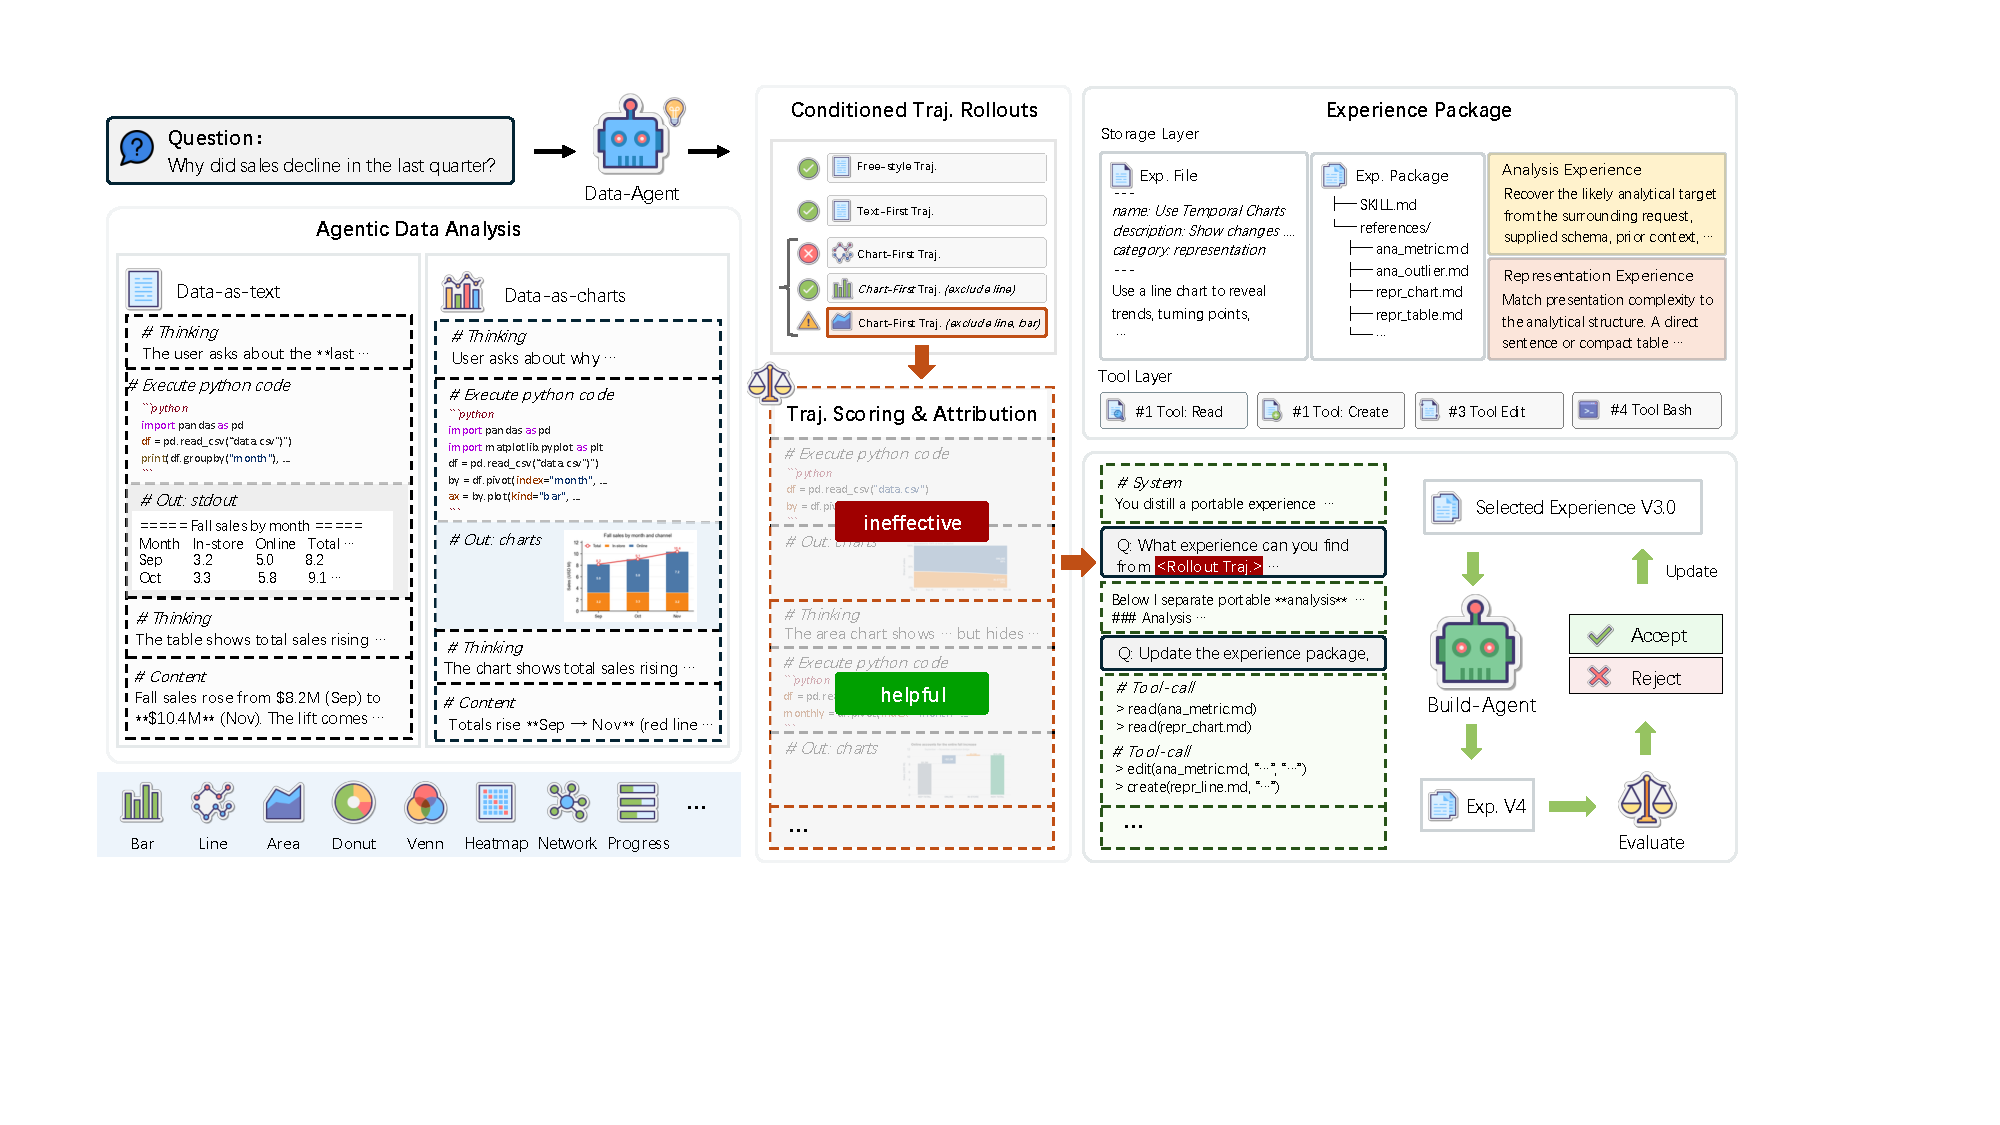
\includegraphics[width=0.98\linewidth]{figures/fig_main_v1.pdf}
\caption{Overall pipeline of \method{}. Conditioned rollouts diversify representation preferences over each \probe{}. A trajectory judge produces outcome scores and step-level attributions. A builder agent distils analysis and representation experiences under a validation gate.}
\label{fig:method}
\end{figure}

\subsection{Storing Experience as Editable Documents}
\label{sec:experience-memory}

\noindent Representation choice depends on the analysis state, so the knowledge that governs it has to stay inspectable and revisable after training ends. We therefore keep experience outside the model as a document store that the agent reads during analysis and a builder revises during distillation. This choice also lets us audit what the agent learned and freeze it before any external evaluation.

\stitle{Two-layer storage.}\quad To make experience readable, editable, and callable on demand, we organise it as a two-layer package. The storage layer is a file-system tree in which an entry document indexes independent experience documents. Each document carries metadata fields \texttt{name}, \texttt{description}, and \texttt{category} together with its content, which supports direct reading, targeted editing, and versioning. The tool layer exposes \texttt{Read}, \texttt{Create}, \texttt{Edit}, and \texttt{Bash} for managing the package. The builder agent uses all four, while the data agent accesses experience only through \texttt{Read}. The data agent first fetches document metadata and then reads relevant content on demand, so context load stays low and grows with task complexity.

\stitle{Analysis and representation experience.}\quad To separate what to compute from how to represent it, we index two experience families under different categories. Analysis experience $\mathcal{E}_{\mathrm{ana}}$ holds reusable rules for selecting, organising, and verifying analytical operations. Representation experience $\mathcal{E}_{\mathrm{repr}}$ holds rules for when intermediate evidence should use text, charts, or a mixture, and for how to consume the resulting evidence in later steps. The two families share the same storage and tool interface, and they are always updated and validated as one package. We write the $v$-th accepted version as $\mathcal{E}^{(v)}=\bigl(\mathcal{E}_{\mathrm{ana}}^{(v)},\mathcal{E}_{\mathrm{repr}}^{(v)}\bigr)$.

\subsection{Distilling Experience from Conditioned Rollouts}
\label{sec:experience-distillation}

\noindent A single rollout per task reveals only the habit the backbone already has, and Section~\ref{sec:probe-findings} shows that this habit is text-heavy for most backbones. Distillation from such data would reproduce the gap we want to close. We therefore force each task to be solved several times under different representation conditions, so the corpus contains chart-led trajectories even for backbones that would never produce them on their own, and outcome differences become attributable to representation choice.

\stitle{Conditioned rollout bundle.}\quad To realise this, we generate multiple trajectories per task while holding the base agent, tools, and interaction budget fixed. Let $p_i=(D_i,q_i,z_i,y_i^{\star})$ denote the $i$-th \probe{}, where the four elements are the data, question, task context, and reference answer. A trajectory generated under representation condition $\rho\in\{\mathrm{U},\mathrm{T},\mathrm{C}_1,\mathrm{C}_2,\mathrm{C}_3\}$ is written $\tau_i^{\rho}$, and each task yields a bundle
\begin{equation}
\mathcal{B}_i=\bigl\{\tau_i^{\mathrm{U}},\tau_i^{\mathrm{T}},\tau_i^{\mathrm{C}_1},\tau_i^{\mathrm{C}_2},\tau_i^{\mathrm{C}_3}\bigr\},
\end{equation}
where $\tau_i^{\mathrm{U}}$ is an unconstrained rollout, $\tau_i^{\mathrm{T}}$ is a text-preferred rollout, and $\{\tau_i^{\mathrm{C}_k}\}_{k=1}^{3}$ are three chart-preferred rollouts. To keep the chart-preferred rollouts from collapsing onto a single visual habit, we enforce type exclusion across them. The second rollout cannot reuse any chart type used by the first, and the third cannot reuse any type used by the first two. This diversifies visual analyses without presuming that any chart type is intrinsically superior.

\stitle{Outcome and step signals.}\quad Bundle-level outcomes alone would tell the builder which trajectory won but not which decision earned the win, so we attach two labels to every trajectory. The outcome scoring function $f_{\mathrm{score}}(\tau_i^{\rho}\mid q_i,y_i^{\star})\!\in\![0,1]$ evaluates the final answer against the reference. The step-level attribution function $f_{\mathrm{attr}}(\tau_i^{\rho}\mid q_i,y_i^{\star})$ labels each key step with a tag in $\{\texttt{Helpful},\texttt{Ineffective},\texttt{Harmful}\}$ and separates the contribution of analytical operations from that of representation choices. Together the two functions tell the builder which behaviours to retain and which to avoid.

\stitle{Insight induction and package revision.}\quad To turn labelled trajectories into transferable rules, we split \probe{} into construction and validation sets so that all trajectories from one task remain in the same split. At each iteration, we sample $b$ tasks from the construction set and feed their bundles and labels to the builder. The builder first performs \textit{insight induction}, comparing trajectories and their attributions to identify transferable analytical and representational patterns. It then performs \textit{package revision}, reading the current package $\mathcal{E}^{(v-1)}$ and either merging new patterns into existing documents or creating fresh entries.

\stitle{Validation-gated update.}\quad An unconstrained builder can overwrite a working document with a pattern that held on one batch only, so every proposal must earn its place. Let $Q(\mathcal{E})$ denote validation performance with package $\mathcal{E}$, and let $\widetilde{\mathcal{E}}^{(v)}$ be the proposal at iteration $v$. The update rule is
\begin{equation}
\mathcal{E}^{(v)}=
\begin{cases}
\widetilde{\mathcal{E}}^{(v)}, & Q(\widetilde{\mathcal{E}}^{(v)})>Q(\mathcal{E}^{(v-1)}),\\[2pt]
\mathcal{E}^{(v-1)}, & \text{otherwise}.
\end{cases}
\label{eq:experience-gate}
\end{equation}
After multiple iterations, the accepted package $\mathcal{E}^{\star}$ is frozen for downstream use. The gate keeps validation performance monotonically non-decreasing and filters proposals that fit a single batch.

\subsection{Consulting Experience inside the Analysis Loop}
\label{sec:online}

\noindent A frozen package pays off only if the agent reaches for it at the moment a representation decision arises. We therefore attach the package to the running analysis loop as a read-only resource, so no extra training, retrieval model, or change to the ReAct interface is needed.

\stitle{Access to the frozen package.}\quad The data agent treats $\mathcal{E}^{\star}$ as external memory. It first receives document metadata, then reads the entries that match the question and the current analysis state. Reading costs a few tool calls and leaves the backbone untouched, so the same package serves every backbone we evaluate.

\stitle{Representation choice at each step.}\quad Analysis experience $\mathcal{E}_{\mathrm{ana}}^{\star}$ guides operation selection and verification, and representation experience $\mathcal{E}_{\mathrm{repr}}^{\star}$ guides whether an intermediate result should use text, charts, or both. Charts therefore enter the loop at the point where the analysis state calls for shape reading, instead of appearing only as a final artefact.

\section{Experiments}
\label{sec:experiments}

\noindent This section evaluates \method{} on three held-out benchmarks that cover analytical report generation, long-horizon exploration, and exact-answer analysis. We describe the benchmarks and evaluation protocol, report main results by capability, and analyse the mechanism through ablations.

\subsection{Benchmarks}
\label{sec:benchmarks}

\noindent To cover the main task forms of agentic data analysis, we adopt three benchmarks with complementary demands and use each benchmark's official protocol.

\stitle{Analytical report generation.}\quad \textbf{DAComp-DA} \citep{lei2025dacomp} contains open-ended tasks over potentially multi-table SQLite databases and requires reports with analysis, conclusions, and visualisations. It is evaluated by Completeness, Accuracy, Insightfulness, Readability, Analytical Depth, Visualisation, and Overall.

\stitle{Long-horizon exploration.}\quad \textbf{DDR-Bench} \citep{liu2026ddrbench} evaluates long-horizon exploration without predefined queries in a 10-K setting over SEC disclosures. It is evaluated by Message-Wise accuracy, Trajectory-Wise accuracy, and Overall.

\stitle{Exact-answer analysis.}\quad \textbf{DSBench} \citep{jing2024dsbench} derives exact-answer analytical tasks from ModelOff competitions with spreadsheet, text, and image inputs. It is evaluated by Task-level Accuracy, Competition-level Accuracy, and Overall.

\subsection{Experimental Setup}
\label{sec:main-exp-setup}

\stitle{Matched agent stack.}\quad To rule out that gains come from tool access, the baseline agent and \method{} share the model version, decoding configuration, system instructions, data access, interaction budget, ReAct loop, and available tools within each backbone. Only \method{} additionally reads the frozen experience package.

\stitle{Isolation of leakage.}\quad All experience distillation uses \probe{} only, and the three benchmarks are held out from experience construction, so downstream numbers measure transfer. Reported prior results are compared only when the split and protocol match.

\stitle{Per-backbone freezing.}\quad Each backbone builds its own package from the same initial structure, and the accepted version is frozen before external evaluation, so no evaluation signal reaches the package.

\subsection{Main Results}
\label{sec:main-results}

\stitle{Analytical report generation.}\quad To verify whether experience-driven chart use improves report-style analysis, we evaluate on DAComp-DA under its official rubric. Table~\ref{tab:dacomp-matrix} compares baseline agents and \method{} across six backbones. Both Analytical Depth and Visualisation improve, and content-correctness metrics move up in tandem. This joint pattern places the improvement inside the analytical process itself and rules out a purely stylistic postprocessing effect. Backbones that essentially never used charts under Free-style now produce reports with substantive visual support. Representation experience $\mathcal{E}_{\mathrm{repr}}$ therefore shifts the agent's habit, and does not simply enable a tool.

\stitle{Long-horizon exploration.}\quad To test whether experience-driven chart use survives long-horizon settings without predefined queries, we evaluate on DDR-Bench 10-K. Table~\ref{tab:downstream-matrix} reports Message-Wise and Trajectory-Wise accuracy. \method{} lifts Trajectory-Wise accuracy, so experience helps the agent maintain coherent exploration across many steps and not only improve isolated messages. Message-Wise accuracy also improves in parallel, so analysis experience $\mathcal{E}_{\mathrm{ana}}$ contributes at both the local and global scale. The pattern of gains on DDR-Bench highlights the value of representation-aware evidence for long-horizon exploration where charts summarise state that pure text loses across steps.

\stitle{Exact-answer analysis.}\quad To check whether \method{} preserves correctness on tasks whose answers must match exactly, we evaluate on the DSBench Data Analysis subset. Table~\ref{tab:downstream-matrix} shows that both Task-level and Competition-level accuracy improve. Since exact-answer tasks penalise vague reasoning, the gains here reflect a tighter analytical policy in which charts serve as intermediate verification, and not as a final narrative artefact. The results extend the effect of experience-driven chart use from generative report tasks to strictly graded analytical tasks.

\begin{table}[t]
\caption{Analytical report generation on DAComp-DA. Higher is better on all metrics. \method{} shares every configuration with the matched baseline except access to $\mathcal{E}^{\star}$.}
\label{tab:dacomp-matrix}
\centering
\small
\setlength{\tabcolsep}{3pt}
\begin{tabular}{@{}llccccccc@{}}
\toprule
Method & LLM Backbone & Comp. & Acc. & Insi. & Read. & Depth & Vis. & Overall \\
\midrule
\multirow{2}{*}{OpenHands} & GPT-5 & 60.98 & 40.30 & 49.39 & 35.51 & 69.80 & 21.40 & 46.99 \\
                          & DeepSeek-V3.1 & 49.88 & 33.25 & 41.66 & 36.00 & 33.20 & 11.00 & 33.87 \\
\midrule
\multirow{2}{*}{DA-Agent} & GPT-5 & 64.23 & 43.81 & 56.89 & 43.59 & 76.80 & 27.44 & 50.84 \\
                         & DeepSeek-V3.1 & 48.74 & 32.97 & 42.43 & 37.25 & 35.00 & 11.45 & 34.33 \\
\midrule
\multirow{4}{*}{Baseline}
& Claude Sonnet 5 & 70.27 & 52.55 & 68.85 & 90.80 & 89.00 & 62.80 & 69.84 \\
& GPT-5.6 Luna & 66.21 & 46.61 & 65.45 & 83.83 & 80.74 & 7.66 & 54.32 \\
& GPT-5.6 Sol & 71.74 & 58.04 & 72.42 & 94.60 & 93.00 & 61.80 & 73.24 \\
& DeepSeek V4.1 Flash & 83.91 & 67.80 & 81.77 & 98.00 & 94.44 & 75.72 & 82.23 \\
\midrule
\multirow{4}{*}{\method{}}
& Claude Sonnet 5 &  &  &  &  &  &  &  \\
& GPT-5.6 Luna & 68.10 & 51.18 & 65.24 & 82.83 & 85.00 & 27.61 & 59.78 \\
& GPT-5.6 Sol &  &  &  &  &  &  &  \\
& DeepSeek V4.1 Flash &  &  &  &  &  &  &  \\
\bottomrule
\end{tabular}
\end{table}

\begin{table}[t]
\caption{Downstream results on DDR-Bench (10-K) and the DSBench Data Analysis subset. Msg. and Traj. denote Message-Wise and Trajectory-Wise accuracy. Task and Comp. denote Task-level and Competition-level accuracy.}
\label{tab:downstream-matrix}
\centering
\small
\setlength{\tabcolsep}{6pt}
\begin{tabular}{@{}llccccccc@{}}
\toprule
 & & \multicolumn{3}{c}{DDR-Bench (10-K)} & & \multicolumn{3}{c}{DSBench} \\
\cmidrule(lr){3-5}\cmidrule(lr){7-9}
Method & LLM Backbone & Msg. & Traj. & Overall & & Task & Comp. & Overall \\
\midrule
\multirow{4}{*}{ReAct}
& Claude Sonnet 4.5 & 77.61 & 60.58 & 69.10 & &  &  &  \\
& GPT-5.1 & 37.12 & 44.25 & 40.69 & &  &  &  \\
& GPT-5.2 & 44.89 & 41.09 & 42.99 & &  &  &  \\
& DeepSeek V3.2 & 60.08 & 38.15 & 49.12 & &  &  &  \\
\midrule
\multirow{2}{*}{Code Interpreter} & GPT-3.5 &  &  &  & & 11.16 & 8.23 & 9.70 \\
& GPT-4o &  &  &  & & 23.82 & 22.65 & 23.24 \\
\midrule
\multirow{2}{*}{AutoGen} & GPT-3.5 &  &  &  & & 20.82 & 13.80 & 17.31 \\
& GPT-4o &  &  &  & & 34.12 & 26.72 & 30.42 \\
\midrule
\multirow{4}{*}{Baseline}
& Claude Sonnet 5 & 61.2 & 52.2 & 56.7 & & 88.47 & 88.42 & 88.45 \\
& GPT-5.6 Luna & 44.5 & 45.1 & 44.8 & & 75.11 & 73.84 & 74.47 \\
& GPT-5.6 Sol & 60.2 & 58.5 & 59.4 & & 89.90 & 89.40 & 89.70 \\
& DeepSeek V4.1 Flash & 64.2 & 59.0 & 61.6 & &  &  &  \\
\midrule
\multirow{4}{*}{\method{}}
& Claude Sonnet 5 &  &  &  & &  &  &  \\
& GPT-5.6 Luna &  &  &  & & 76.72 & 76.25 & 76.49 \\
& GPT-5.6 Sol &  &  &  & &  &  &  \\
& DeepSeek V4.1 Flash &  &  &  & &  &  &  \\
\bottomrule
\end{tabular}
\end{table}

\begin{table}[t]
\centering
\begin{minipage}[t]{0.52\textwidth}
\centering
\captionof{table}{Distillation procedure on DAComp-DA.}
\label{tab:ablation-construction}
\small
\setlength{\tabcolsep}{5pt}
\begin{tabular}{@{}lccc@{}}
\toprule
Variant & Acc. & Vis. & Overall \\
\midrule
Matched baseline & 46.61 & 7.66 & 54.32 \\
One-step distillation &  &  &  \\
w/o conditioned rollouts &  &  &  \\
w/o validation gate &  &  &  \\
\method{} & 51.18 & 27.61 & 59.78 \\
\bottomrule
\end{tabular}
\end{minipage}\hfill
\begin{minipage}[t]{0.44\textwidth}
\centering
\captionof{table}{Experience types on DAComp-DA.}
\label{tab:ablation-experience-types}
\small
\setlength{\tabcolsep}{5pt}
\begin{tabular}{@{}lccc@{}}
\toprule
Variant & Acc. & Vis. & Overall \\
\midrule
Analysis only &  &  &  \\
Representation only &  &  &  \\
\method{} & 51.18 & 27.61 & 59.78 \\
\bottomrule
\end{tabular}
\end{minipage}
\end{table}

\subsection{Ablation Studies and Mechanism Analysis}
\label{sec:ablations}

\stitle{Ablation protocol.}\quad To locate which mechanism inside \method{} drives the gains, we run all ablations on DAComp-DA with the same backbone, ReAct loop, tool interface, interaction budget, and evaluator. We report Acc., Vis., and Overall, which measure analytical correctness, visual evidence quality, and aggregate performance. Each ablation changes only the component under study.

\FloatBarrier

\begin{wrapfigure}[16]{r}{0.44\textwidth}
\centering
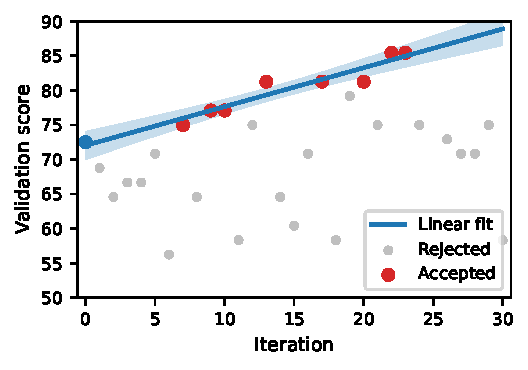
\includegraphics[width=\linewidth]{figures/experience_distillation_convergence_v2.pdf}
\caption{Validation trajectory during experience distillation. The gate admits only proposals that improve held-out performance.}
\label{fig:experience-convergence}
\end{wrapfigure}

\stitle{Iterative distillation.}\quad To test whether the iterative construction of experience matters, we compare \method{} against one-step distillation that builds the package from the full trajectory corpus in a single builder call. Table~\ref{tab:ablation-construction} shows that iterative construction yields a better balance across analytical correctness and visual evidence quality. Iteration allows the builder to refine documents in light of newly labelled trajectories and to remove entries that do not transfer, so the resulting package stays compact and reusable.

\stitle{Rollout diversity and validation gate.}\quad To attribute the gain to the two mechanisms in the training loop, we ablate conditioned rollouts and the validation gate. Removing conditioned rollouts collapses the diversity of representation choices seen during distillation and pulls the package back toward text-only patterns. Removing the validation gate lets noisy edits accumulate and lowers Overall. Both mechanisms therefore contribute to the final policy.

\stitle{Two experience families.}\quad To separate the roles of analysis and representation experience, we retain documents from only one family. Table~\ref{tab:ablation-experience-types} shows that analysis experience mainly moves Acc., while representation experience mainly moves Vis. Combining the two families reaches the best Overall. Analytical operation selection and evidence representation therefore act as complementary contributions, and not as redundant ones.

\stitle{Optimisation dynamics.}\quad To visualise how experience reshapes agent behaviour and how the validation gate stabilises training, Figure~\ref{fig:experience-convergence} tracks the retained package's validation score across iterations. The gate keeps the trajectory monotonically non-decreasing and filters proposals that overfit to a single batch. Together with the ablations, this shows that \method{} builds up an increasingly compact policy for representation-aware analysis.

\FloatBarrier
\section{Related Work}
\label{sec:related}

\stitle{Data agents.}\quad LLM-driven data agents follow a plan, execute, observe, and revise loop over structured data. Representative systems couple reasoning with executable environments and cover heterogeneous analysis. DS-Agent \citep{guo2024dsagent} retrieves historical cases inside an executable loop, Data Interpreter \citep{hong2025datainterpreter} organises tasks as dynamic directed acyclic graphs, AIDE \citep{jiang2025aide} models solution development as tree search over code, DS-STAR \citep{nam2025dsstar} adds sufficiency verification, AutoKaggle \citep{li2025autokaggle} adopts multi-agent division of labour, DeepAnalyze \citep{zhang2025deepanalyze} trains an end-to-end data science model, and InsightBench \citep{sahu2025insightbench} extends evaluation to open-ended business insight generation. These systems keep the analytical loop text-centric and treat charts primarily as report artefacts. \method{} instead makes charts a first-class intermediate action of the analytical loop.

\stitle{Chart generation and understanding.}\quad One line of work optimises the production or reading of a single chart. LIDA \citep{dibia2023lida}, MatPlotAgent \citep{yang2024matplotagent}, ChartMimic \citep{yang2025chartmimic}, AMACE \citep{namgoong2025amace}, MultiVis-Agent \citep{lu2026multivisagent}, and ChartOptimiser \citep{wang2025chartoptimiser} improve chart generation through rendered feedback, multi-agent collaboration, and intent-aware design. UniChart \citep{masry2023unichart}, ChartLlama \citep{han2023chartllama}, and ChartBench \citep{xu2023chartbench} advance chart reading through specialised training, and DePlot \citep{liu2023deplot}, MatCha \citep{liu2023matcha}, and TinyChart \citep{zhang2024tinychart} strengthen numerical analysis through derendering and programmatic reasoning. These methods assume that the chart or the plotting request is already fixed. \method{} decides when a chart should exist at all inside an analytical trajectory.

\stitle{Representation choice for reasoning.}\quad A recent line of work studies how the choice of textual, tabular, or visual representation affects reasoning. ChartAgent \citep{kaur2026chartagent} and Charts-of-Thought \citep{das2025chartsofthought} combine visual tools with structured reasoning, FRES \citep{zhou2025fres}, FormatMatters \citep{ho2026formatmatters}, and TableDART \citep{xing2026tabledart} compare textual, image, and chart formats, and EvidFuse \citep{lin2026evidfuse} builds visual evidence on demand. These methods pick among predefined formats or attach visual tools with fixed rules. \method{} learns state-dependent representation choice from labelled analytical trajectories, so text and chart evidence are selected as the analysis unfolds, and not fixed at task setup.

\section{Conclusion}
\label{sec:conclusion}

\noindent We study whether charts can serve as internal epistemic actions inside a data agent's analytical loop. \probe{} shows that current agents extract sufficient evidence from self-generated charts, yet plotting access alone does not translate into consistent chart use. Charts and text play complementary roles across task slices, with charts stronger on temporal, pattern, and anomaly reasoning and text stronger on precise reading and conditional verification. Motivated by these findings, \method{} distils analysis experience $\mathcal{E}_{\mathrm{ana}}$ and representation experience $\mathcal{E}_{\mathrm{repr}}$ from conditioned trajectory rollouts using outcome scoring $f_{\mathrm{score}}$ and step-level attribution $f_{\mathrm{attr}}$, and retains only experiences that pass a validation gate. On three held-out benchmarks with six LLM backbones, \method{} activates chart use, improves analytical accuracy, and lifts visual evidence quality without touching model parameters. These results position representation choice as part of the analytical policy, and not as a cosmetic output stage.

\bibliography{iclr2027_conference}
\bibliographystyle{iclr2027_conference}

\appendix

\section{Complete \probe{} Slice Results}
\label{app:slices}

\noindent We report the full slice tables that support the findings in Section~\ref{sec:probe-findings}. A task may carry multiple analytical-operation labels and one primary cognitive-operation label.

\begin{table}[h]
\caption{Scores by analytical operation.}
\label{tab:operation-slices}
\centering
\small
\setlength{\tabcolsep}{4pt}
\begin{tabular}{@{}lrrrrr@{}}
\toprule
Slice & $n$ & No-tool & Text & Chart & Free-style \\
\midrule
Filtering             & 109 & 0.257 & 0.752 & 0.752 & 0.755 \\
Feature derivation    & 116 & 0.257 & 0.739 & 0.752 & 0.744 \\
Aggregation           & 163 & 0.305 & 0.773 & 0.791 & 0.781 \\
Normalisation         &  21 & 0.143 & 0.571 & 0.512 & 0.583 \\
Sorting               &  22 & 0.284 & 0.818 & 0.830 & 0.784 \\
Alignment or joining  &   8 & 0.188 & 0.719 & 0.563 & 0.719 \\
Temporal change       &  37 & 0.237 & 0.757 & 0.838 & 0.757 \\
Distributional stats. &   1 & 1.000 & 1.000 & 1.000 & 1.000 \\
Statistical inference &  10 & 0.200 & 0.925 & 0.900 & 0.900 \\
Forecasting           &   3 & 0.000 & 1.000 & 1.000 & 1.000 \\
\bottomrule
\end{tabular}
\end{table}

\begin{table}[h]
\caption{Scores by primary cognitive operation.}
\label{tab:cognitive-slices}
\centering
\small
\setlength{\tabcolsep}{4pt}
\begin{tabular}{@{}lrrrrr@{}}
\toprule
Slice & $n$ & No-tool & Text & Chart & Free-style \\
\midrule
Lookup                       & 12 & 0.146 & 0.604 & 0.521 & 0.521 \\
Scan and selection           & 24 & 0.219 & 0.958 & 0.958 & 0.958 \\
Comparative judgment         & 69 & 0.366 & 0.801 & 0.783 & 0.808 \\
Pattern recognition          & 54 & 0.306 & 0.769 & 0.833 & 0.764 \\
Relational explanation       & 17 & 0.221 & 0.706 & 0.735 & 0.765 \\
Multidimensional integration & 20 & 0.150 & 0.575 & 0.650 & 0.600 \\
Conditional reasoning        &  4 & 0.813 & 1.000 & 0.750 & 1.000 \\
\bottomrule
\end{tabular}
\end{table}

\end{document}
